\clearpage{\pagestyle{empty}\cleardoublepage}
\chapter{L'algoritmo di minimizzazione}\label{Chap:Algo}
Per la risoluzione del problema utilizziamo la tecnica del Branch and Bound, la quale si basa sulla scomposizione del problema originale in sottoproblemi (nodi), pi� semplici da risolvere.\\
Per limitare il numero di nodi da esaminare si associa ad ogni nodo un ``lower bound'', ossia un limite inferiore, che indica una stima per difetto del valore di tutte le soluzioni complete ottenibili come discendenti di quel nodo. Anche un ``upper bound'' deve essere noto e viene usato come termine di confronto per i lower bounds dei nodi. L'upper bound � il valore della migliore soluzione trovata sinora. Se un nodo dell'albero ha un lower bound maggiore o uguale all'upper bound corrente, esso viene chiuso, cio� viene eliminato dalla lista dei nodi aperti. Infatti tutte le soluzioni complete che si otterrebbero da esso avrebbero un valore non migliore del valore della soluzione ottima corrente. La stessa cosa avviene se si dimostra che il consumo di risorsa sul nodo non pu� essere inferiore al budget perch� le soluzioni complete che sottrarrebbero non possono essere ammissibili .

\section{Calcolo del lower bound}

Per il calcolo del lower bound (\verb|LB|), una prima idea � quella di ignorare il vincolo del $Budget$ affinch� il problema diventi risolvibile in tempo polinomiale $O(N^{3})$, dato che si riduce a un linear assignement problem. Questo pu� essere risolto usando l'algoritmo descritto in \cite{shortLap}, disponibile in rete come libreria \verb|lap.c|.\\
Il linear assignement problem, � definito come segue:\\
\textsc{Dati}:
\begin{itemize}
	\item $|V_{1}|=n$ persone e $|V_{2}|=n$ compiti
	\item $c_{ij}$ costo di attribuzione del compito $j \in V_{2}$ alla persona $i \in V_{1}$
\end{itemize}
\textsc{Variabili}:
	\begin{equation*}
		x_{i,j}=
			\begin{cases}		
				1& \text{compito $j \in V_{2}$ a persona $i \in V_{1}$},\\		
				0& \text{altrimenti}.
			\end{cases}
	\end{equation*}
\textsc{Vincoli}:
\begin{itemize}
	%1)
	\item Una persona deve essere associata a un solo progetto:\hfill
		\begin{equation}\label{eq:prog_lav}
			\displaystyle\sum_{j \in V_{2}}x_{ij}=1 \qquad i \in V_{1}
		\end{equation}
	%2)
	\item Un progetto deve essere associato a una sola persona:\hfill
		\begin{equation}\label{eq:lav_prog}
			\displaystyle\sum_{i \in V_{1}}x_{ij}=1\qquad j \in V_{2}
		\end{equation}
	%3)
	\item Vincolo di budget\hfill
		\begin{equation}\label{eq:budget}
			\ds\sum_{i \in V_{1}}\ds\sum_{j \in V_{2}} r_{ij} x_{ij} \leq B
		\end{equation}
\end{itemize}
\textsc{Obiettivo}:
\begin{itemize}
	\item si vuole minimizzare il costo totale:
		\begin{equation}
			\min\ \ds\sum_{i \in V_{1}}\ds\sum_{j \in V_{2}} c_{ij} x_{ij} 
		\end{equation}
\end{itemize}
Il calcolo del lower bound, avviene nella funzione \verb|ProcessBnode| da parte della funzione \verb|CalcoloLB|, che riceve: il nodo corrente \verb|N|, i dati del problema \verb|PD|, e la soluzione migliore (Best Solution) \verb|BS|.
Nella struttura dati del nodo, \verb|N.LB|, viene salvato il valore del lower bound calcolato tramite la funzione \verb|lap|, la quale riceve come input la dimensione del problema, \verb|dim| e la matrice dei costi \verb|assigncost|, e fornisce come output la soluzione stessa, descritta attraverso i due vettori \verb|LBcolsol| e \verb|LBrowsol| che riportano, rispettivamente, la persona a cui � assegnato ogni progetto e il progetto assegnato a ogni persona.

\section{Penalit� Lagrangiane}\label{sec:Penalit�Lagrangiane}

Per evitare di generare tramite branching nodi che non possono portare un miglioramento, vengono inserite condizioni note come penalit� lagrangiane. Se il costo ridotto di una cella della matrice dei costi, � maggiore dell'intervallo esistente tra l'upper bound e il lower bound, allora � possibile scartare tale cella fissando la corrispondente cella nella matrice dei vincoli a zero. Questo perch� tale costo stima per difetto l'incremento che la funzione obiettivo subirebbe forzando la corrispondente variabile a 1.

%==========================================================================
%		Secondo lower bound Zaino a scelta multipla, tolto in un secondo momento non controllato!
%==========================================================================
%\section{Calcolo del secondo lower bound}
%Nel calcolo del primo lower bound abbiamo trascurato il vincolo del budget (cfr. (\ref{eq:budget}) a Pagina \pageref{eq:budget}), mentre per il calcolo del secondo, abbiamo trascurato il vincolo che associa a ogni persona a un solo progetto (cfr. (\ref{eq:lav_prog}) a Pagina \pageref{eq:lav_prog}).\\
%In questo modo, si ottiene il problema dello zaino a scelta multipla, risolvibile con la procedura: \verb|fmcknap.c|. \cite{caselli,Pis95Mcknap}\\
%%Il codice \verb|fmcknap.c|, risolve il problema della massimizzazione, di conseguenza il nostro problema deve essere descritto come:
%Il problema dello zaino a scelta multipla � definito come:\\
%\textsc{Variabili}:
%	\begin{itemize}
%		\item $x_{ij}\in \left\{ 0,1\right\}$
%	\end{itemize}
%\textsc{Vincoli}:
%	\begin{itemize}
%		\item $\ds\sum_{j} x_{ij}=1 \qquad \forall_{i}$
%		\item $\ds\sum_{ij} r_{ij}x_{ij} \leq B$
%	\end{itemize}
%\textsc{Obiettivo}:
%	\begin{itemize}
%		\item  $\ds\sum_{ij} a_{ij}x_{ij}$
%	\end{itemize}
%Per ottenere un'istanza del problema dello zaino a scelta multipla, servono questi passaggi:
%\begin{itemize}
%	\item $min \ds\sum_{ij} \widetilde{c}_{ij} x_{ij} \quad\Rightarrow\quad - max \ds\sum_{ij} -\widetilde{c}_{ij} x_{ij}$\\
%	Dove $\widetilde{c}_{ij}$, rappresenta la matrice dei costi a cui sono stati sottratti i vettori $u_{i}$ e $v_{j}$: $\widetilde{c}_{ij}= c_{ij}-u_{i}-v_{j}$.
%	\item trovo il minimo della matrice definito come: $K = -min\ -\widetilde{c}_{ij}$
%	\item sommo il valore $-K$ a tutti i valori della matrice $\widetilde{c}_{ij}$
%	\item pongo $a_{ij}=\widetilde{c}_{ij} - K$
%\end{itemize}
%===========================================================
%		Fine mcknap
%===========================================================
\section{Calcolo dell'upper bound}

Per il calcolo dell'upper bound (\verb|UB|), viene creata una nuova matrice $\gamma$~(\verb|gamma|) che contiene una combinazione convessa dei costi e del consumo di risorsa. Essa � quindi definita come $\gamma_{ij}=\alpha \cdot c_{ij}+\left(1-\alpha \right)\cdot r_{ij}$; dove $c_{ij}$ � la matrice dei costi, mentre $r_{ij}$ quella delle risorse. Sulla matrice $\gamma$, viene eseguita la funzione \verb|lap|, la quale restituisce il vettore delle soluzioni \verb|rowsolGamma|; grazie alle coordinate fornite dal vettore, viene calcolato il costo sulla matrice dei costi, e il consumo sulla matrice delle risorse.
\begin{center}
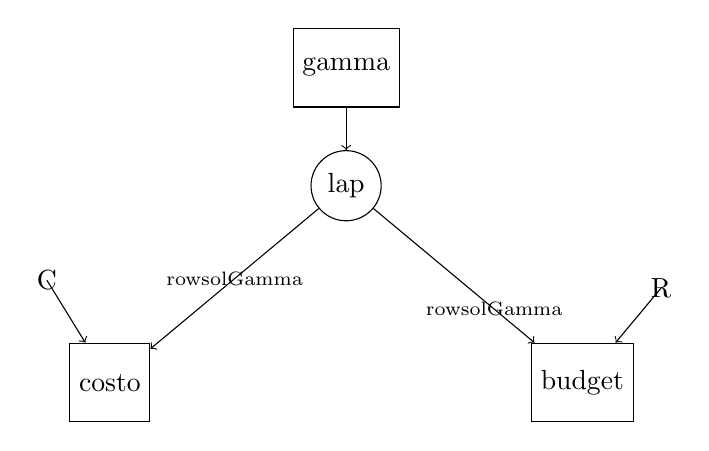
\begin{tikzpicture}
% Nodo Gamma
\draw(0,0)node[minimum height=1cm, minimum width=1cm,draw](node gamma){gamma}
		 % Nodo lap
		 (0,-1.5)node[minimum height=0.5cm, minimum width=0.5cm,draw,circle](node lap){lap}
		 % Nodo matrice costi
		 (-3,-4)node[minimum height=1cm, minimum width=1cm,draw](node cost){costo}
		 % Nodo matrice risorse
		 (+3,-4)node[minimum height=1cm, minimum width=1cm,draw](node bud){budget};

\draw[->](node gamma)--(node lap);
% Freccia da lap a costi
\draw[->](node lap)--(node cost)node[midway]{\scriptsize{rowsolGamma}};
% Matrice costi c freccia piccola
\draw[->](-3.8,-2.7)--(node cost)node[at start]{C};
% Freccia da lap a budget
\draw[->](node lap)--(node bud)node[near end]{\scriptsize{rowsolGamma}};
% Freccia matrice risorse piccola
\draw[->](4,-2.8)--(node bud)node[at start]{R};
\end{tikzpicture}
\end{center}

A ogni iterazione, il suo costo (\verb|UB|), viene confrontato con l'upper bound globale nella struttura dati \verb|BestSolution|, se � minore, viene aggiornata la migliore soluzione trovata fino a quel momento.\\

Infine $\alpha$ � un parametro che varia tra 0 e 1. Valutata (sempre con \verb|lap.c|) la soluzione ottima rispetto a gamma, si pu� calcolarne il consumo totale di risorsa e il costo. Se il consumo � minore o uguale al budget, questo significa che si � dato troppo peso al consumo di risorsa. Quindi il parametro $\al$ cresce come segue:
\begin{align*}
	\al_{m} &= \al\\
	\al_{M} &= \al_{M}\\
	\al     &= \ds\frac{1}{2}\al+\frac{1}{2}\al_{M}.
\end{align*}
Se il consumo � maggiore del budget, questo significa che si � dato troppo poco peso al consumo di risorsa. Quindi il parametro $\alpha$ si modifica come segue:
\begin{align*}
	\al_{M} &= \al\\
	\al_{m} &= \al_{m}\\
	\al     &= \ds\frac{1}{2}\al+\frac{1}{2}\al_{m}.
\end{align*}
L'aggiornamento di $\al$ viene eseguito per 10 iterazioni. Il valore iniziale di $\al$ � 1 (cio� si minimizza il solo consumo di risorsa). Se la soluzione corrispondente ha un consumo superiore al budget B, possiamo concludere che nessuna soluzione del nodo corrente � ammissibile, quindi il nodo si pu� chiudere senza altre elaborazioni.\\
In Pseudocodice \ref{UB} viene mostrata la logica del calcolo.
%Sulla matrice $\gamma$, viene eseguita la funzione \verb|lap|, la quale restituisce il vettore delle soluzioni \verb|rowsolGamma|; grazie alle coordinate fornite dal vettore, viene calcolato il costo sulla matrice dei costi, e il consumo sulla matrice delle risorse.
%\begin{center}
%\begin{tikzpicture}
%% Nodo Gamma
%\draw(0,0)node[minimum height=1cm, minimum width=1cm,draw](node gamma){gamma}
%		 % Nodo lap
%		 (0,-1.5)node[minimum height=0.5cm, minimum width=0.5cm,draw,circle](node lap){lap}
%		 % Nodo matrice costi
%		 (-3,-4)node[minimum height=1cm, minimum width=1cm,draw](node cost){costo}
%		 % Nodo matrice risorse
%		 (+3,-4)node[minimum height=1cm, minimum width=1cm,draw](node bud){budget};
%
%\draw[->](node gamma)--(node lap);
%% Freccia da lap a costi
%\draw[->](node lap)--(node cost)node[midway]{\scriptsize{rowsolGamma}};
%% Matrice costi c freccia piccola
%\draw[->](-3.8,-2.7)--(node cost)node[at start]{C};
%% Freccia da lap a budget
%\draw[->](node lap)--(node bud)node[near end]{\scriptsize{rowsolGamma}};
%% Freccia matrice risorse piccola
%\draw[->](4,-2.8)--(node bud)node[at start]{R};
%\end{tikzpicture}
%\end{center}
%
%A ogni iterazione, il suo costo (\verb|UB|), viene confrontato con l'upper bound globale nella struttura dati \verb|BestSolution|, se � minore, viene aggiornata la migliore soluzione trovata fino a quel momento.\\
\begin{lstlisting}[caption={Calcolo dell'upper bound},label=UB]
CalcoloUB(Nodo, PD, BS)
{
    alpha = 0.5;
    alpham = 0.0;
    alphaM = 1.0;
   
    for (k=0; k<ITERAZIONI; k++) {
        for (i=0; i<dim; i++)
           for (j=0; j<dim; j++)
              gamma[i][j] = alpha*assigncost[i][j]+(1-alpha)*risorse[i][j];
        
        minimoConsumoRisorse = lap (dim, gamma, rowsolGamma, colsolGamma);

        // Calcolo costi
        costo = 0.0;
        for ( i=0; i<dim; i++ )
                costo += assigncost[i][pta->BNinfo.UBrowsol[i]];
        
				// Calcolo del consumo
        consumo = 0.0;
        for ( i=0; i<dim; i++ )
                consumo += risorse[i][pta->BNinfo.UBrowsol[i]];
                
        if ( consumo <= budget ) {
            alphaTemp = alpha;
            alpha = alpha/2 + alphaM/2;
            alpham = alphaTemp;
            if ( costo<pBS->UB )
                pta->BNinfo.UB = costo;
        }
        else {
            alphaTemp = alpha;
            alpha = alpha/2 + alpham/2;
            alphaM = alphaTemp;
        }    
    }    
}
\end{lstlisting}

\section{Strategia di branching}

La strategia di branching consiste nel fissare una variabile ancora libera a 0 oppure a 1. La variabile viene scelta confrontando la soluzione associata al lower bound e quella associata all'upper bound, cio� i due vettori \verb|LBrowsol| e \verb|UBrowsol|. Se i due bound differiscono, le due soluzioni sono diverse. Si osservano le diversit� e si considera la prima variabile presente nella soluzione dell'upper bound e assente in quella del lower bound. La figura seguente illustra un esempio: le matrici rappresentano le soluzioni associate al lower bound (a sinistra) e all'upper bound (a destra). A destra di ogni matrice compaiono i vettori \verb|LBrowsol| e \verb|UBrowsol| che contengono, per ogni riga, l'indice della colonna in cui compare un 1.
\begin{equation*}\label{eq:mat}
\begin{array}{|c|c|c|c|}
\hline
 	& 1 &  & \\
\hline
 1&   &  & \\
\hline
 	&   &  &1 \\
\hline
 	&   &1 &\\
\hline
\end{array} 
\Leftarrow \verb|LBrowsol| \Rightarrow
\begin{array}{|c|}
\hline
 	2\\
\hline
  1\\
\hline
 	4\\
\hline
 	3\\
\hline
\end{array}
\quad
\begin{array}{|c|c|c|c|}
\hline
 	& 1 &  & \\
\hline
 1&   &  & \\
\hline
 	&   & 1 &\textcolor{red}{X} \\
\hline
 	&   & &1\\
\hline
\end{array} 
\Leftarrow \verb|UBrowsol| \Rightarrow
\begin{array}{|c|}
\hline
 	2\\
\hline
  1\\
\hline
 	3\\
\hline
 	4\\
\hline
\end{array}
\end{equation*}

Una volta definito il punto di branching, la funzione \verb|DeriveBnode| crea due figli, copiando nel figlio le informazioni del problema padre e forzando la variabile di branching a 1 nel primo figlio, a 0 nel secondo.

\begin{lstlisting}[caption={DeriveBnode},label=DBN]
DeriveBnode (father, f, son)
{
    // Copio la matrice dei vincoli da padre in figlio
    for (i=0; i<father->BNinfo.dim; i++)
        for (j=0; j<father->BNinfo.dim; j++)
                son->BNinfo.vincoli[i][j] = father->BNinfo.vincoli[i][j];
    
    // Inserisco le informazioni di branching 
    if ( f==1 ) {
        // Fisso a 0 tutti i valori contenuti nella colonna della cella
        // di branching tranne quello della cella stessa.
        son->BNinfo.vincoli[father->branch.i][father->branch.j] = 1;
        for (i=0; i<father->BNinfo.dim; i++)
            if (i != father->branch.i)
                son->BNinfo.vincoli[i][father->branch.j] = 0;

        // Fisso a 0 tutti i valori contenuti nella riga della cella
        // di branching tranne quello della cella stessa.
        for (j=0; j<father->BNinfo.dim; j++)
            if (j != father->branch.j)
                son->BNinfo.vincoli[father->branch.i][j] = 0;
    }    
    else
        son->BNinfo.vincoli[father->branch.i][father->branch.j] = 0;
}
\end{lstlisting}

\section{Strategia di visita dell'albero}

Le strategie di visita implementate sono tre:
\begin{itemize}
	\item depth first search, ovvero in profondit�
	\item breadth first search, ovvero in ampiezza
	\item best first search
\end{itemize}

\subsection{Depth First Search}\label{sec:DepthFirstSearch}

Questa strategia, inserisce il nodo \verb|N| in cima alla lista \verb|BT| dei nodi aperti.\\
Sviluppa, quindi, l'albero in profondit�, partendo dalla radice ed arrivando fino alle foglie. Ad ogni iterazione l'algoritmo sceglie di esplorare uno tra i nodi figli del nodo appena esplorato. Se questo non ha figli, l'algoritmo passa al nodo di pi� basso livello non ancora esplorato.\\
Quindi si esplora un ramo ancora prima di generare quelli successivi.
Siccome i nodi vengono inseriti sempre dalla cima, per poter ottenere la DFS occorre inserire ogni nuovo nodo in cima alla lista.
\begin{lstlisting}[caption={Depth First Search},label=DFS]
if (VisitStrategy == DEPTH_FIRST)
{
	inslista(N,primolista(BT),BT);
}
\end{lstlisting}

\subsection{Breadth First Search}\label{sec:BreadthFirstSearch}

Questa strategia, inserisce il nodo \verb|N| in coda alla lista \verb|BT| dei nodi aperti.\\
Sviluppa, quindi, l'albero in larghezza, considerando prima tutti i nodi dello stesso livello per poi passare a quelli del livello sottostante.
Si inizia calcolando l'upper bound del nodo radice, generando tutti i suoi figli e calcolando i corrispondenti upper bound. Vengono quindi generati tutti i figli di ogni figlio della radice, e cos� via, esplorando sempre tutti i nodi di un livello prima di passare al livello successivo.

\begin{lstlisting}[caption={Depth First Search},label=BFS]
if (VisitStrategy == BREADTH_FIRST)
{
	inslista(N,succlista(ultimolista(BT),BT),BT);
}
\end{lstlisting}

\subsection{Best First Search}\label{sec:BestFirstSearch}

Questa strategia, mantiene la lista dei problemi aperti ordinata per bound crescente. Quindi inserisce il nuovo nodo prima del primo problema peggiore di esso.\\
Ad ogni iterazione l'algoritmo sceglie di esplorare uno tra i nodi a cui � associato il migliore bound della soluzione ottima.

\begin{lstlisting}[caption={Depth First Search},label=BestFS]
if (VisitStrategy == BEST_FIRST)
{
  pos = primolista(BT);
  while (! finelista(pos, BT) )
  {
      if ( pos->BNinfo.LB > pta->BNinfo.LB )
          break;
      pos = succlista(pos,BT);
  }
  inslista(pta,pos,BT);
}
\end{lstlisting}
